\chapter{New Material on Gradient Dynamics and Energy Functions}
\chapterauthor{Scott Hotton, Jeff Yoshimi}

% Break out sections. First, gradient dynamics. Do it intuitively. Explain how it is our main powerhouse for learning in the weight space, but also used to understand main dynamics using energy functions, as in Hopfield
% I have a fair number of notes with Scott on this to integrate as well.

\subsection{Dynamical systems from potential functions}

   A potential function is a smooth scalar field $V \colon \bf{R}^N \to 
\bf{R}$ which is used to perform gradient descent (see section 
\ref{sect_gradient_descent}). The gradient is a first order 
differential operator of functions from $\bf{R}^N$ to $\bf{R}$.  It is often
written as a vector with $N$ entries that are partial derivatives:
\begin{equation*}
   \nabla V(\mathbf{x}) = \left( \dfrac{\partial}{\partial x_1} V(\mathbf{x}),
\ldots, \dfrac{\partial}{\partial x_N} V(\mathbf{x}) \right)^T
\end{equation*}
The gradient tells us the direction in which the slope of the potential 
function is steepest, the direction in which $V$ increases the fastest.  The 
opposite direction is the one in which $V$ decreases the fastest.  

   A gradient dynamical system, also known as a gradient flow, is the solution 
to a differential equation that is obtained by using the gradient operator with
a potential function.  The state of the system is given by a point $\mathbf{x} 
\in \bf{R}^N$.  A gradient flow, is the solution to the differential equation 
obtained by setting the rate of change in $\mathbf{x}$ equal to the negative to 
the gradient of $V$ at $\mathbf{x}$:
\begin{equation}
   \dot{\mathbf{x}} = -\nabla V(\mathbf{x}) 
\end{equation}
No matter where $\mathbf{x}$ is in $\bf{R}^N$ it moves in the direction of
steepest descent of the potential function.  So the local minima of $V$ are 
attracting fixed points of a gradient flow.  All of the points in a small 
enough neighborhood of a local minimum of $V$ must converge to the local 
minimum.  The local maxima are repelling fixed points of a gradient flow.  All 
of the points in a small enough neighborhood of a local maximum (except for 
the local maximum itself) must move away from the local maximum.  

   At a local minimum or a local maximum there is no direction of steepest
descent so the gradient at these points has no direction, it is the zero 
vector.  In fact all of the fixed points of a gradient flow are either where 
the gradient is the zero vector or the gradient is undefined.  If the gradient 
is defined and not zero then $\mathbf{x}$ moves in the opposite direction of 
the gradient.  So long as the gradient is defined at the point $\mathbf{x}$ it
only does not move when the gradient is the zero vector.  The places where the 
gradient is zero or undefined are known as the critical points of the potential 
function.

   The matrix of second order partial derivatives
\begin{equation*}
-
\begin{pmatrix}
\dfrac{\partial^2}{\partial x_1^2}\, V(\mathbf{x}) &
\dfrac{\partial^2}{\partial x_1 \, \partial x_2}\, V(\mathbf{x}) &
\ldots & \dfrac{\partial^2}{\partial x_1 \partial x_N}\, V(\mathbf{x})  \\[4mm]
\dfrac{\partial^2}{\partial x_2 \, \partial x_1}\, V(\mathbf{x}) &
\dfrac{\partial^2}{\partial x_2^2}\, V(\mathbf{x}) &
\ldots & \dfrac{\partial^2}{\partial x_2\,  \partial x_N}\, V(\mathbf{x})  
\\[4mm]
   \vdots & \vdots & \ddots & \vdots \\[4mm]
\dfrac{\partial^2}{\partial x_N \, \partial x_1}\, V(\mathbf{x}) &
\dfrac{\partial^2}{\partial x_N \, \partial x_2}\, V(\mathbf{x}) &
\ldots & \dfrac{\partial^2}{\partial x_N^2}\, V(\mathbf{x})  \\[4mm]
\end{pmatrix}
\end{equation*}
is called the Hessian of $V$.  The entries of the $n^{\mathrm{th}}$ row of the
Hessian are the partial derivatives, with respect to $x_n$, of the entries of 
$-\nabla V(\mathbf{x})$.  The Hessian is a symmetric matrix because of the 
equality of mixed partial derivatives.
\begin{equation*}
\dfrac{\partial^2}{\partial x_j \, \partial x_k}\, V(\mathbf{x}) 
=
\dfrac{\partial^2}{\partial x_k \, \partial x_j}\, V(\mathbf{x}) 
\end{equation*}
for all $j$, $k \in \{1, \ldots, N\}$.  Since the Hessian is symmetric it does 
does not have complex conjugate pairs of eigenvalues.  All of its eigenvalues 
are real numbers. 

   If the determinant of the Hessian is zero then its called a degenerate
Hessian, otherwise its called nondegenerate.  Since the determinant of a
matrix is the product of its eigenvalues none of the eigenvalues of a 
nondegenerate Hessian can be zero.  When all of the second order partial 
derivatives are defined at a critical point of the potential function and the 
Hessian is nondegenerate then the critical point is either a minimum, a 
maximum, or a saddle point.  

   If all of the eigenvalues of the Hessian at a critical point are positive 
then the critical point is a local minimum.  If all of the eigenvalues of the 
Hessian at a critical point are negative then the critical point is a local 
maximum.  If some of the eigenvalues are positive and all of the other 
eigenvalues are negative then the critical point is a saddle point of the 
potential function.  This is a multidimensional version of the second 
derivative test from single variable calculus.  The eigenvectors for different 
eigenvalues of the Hessian are orthogonal.

   The attracting fixed points are the only attracting sets for a gradient 
flow.  For instance there are no attracting periodic orbits since we can not 
return to our starting point when we are always descending down the graph of 
$V$.  

   Aside from the fixed points, the orbits of a gradient flow are orthogonal to
each level hypersurface of $V$ that the orbits pass through.  The basin of 
attracting for the attracting fixed points are connected open sets in $\bf{R}^N$ 
with piecewise smooth boundaries.  Under a gradient flow every point in 
$\bf{R}^N$ is either in the basin of attraction of an attracting fixed point, in
the boundary of the basin of attraction, or it goes off to infinity.  The 
repelling fixed points and saddle nodes are located in the boundaries of the 
basins of attracting for the attracting fixed points.  

\begin{figure}[ht]
\centering
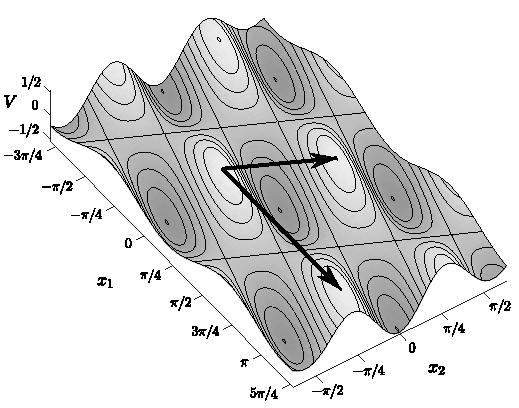
\includegraphics[scale=1.20]{./images/Gradient1.pdf}
\caption{The graph of the potential function $V( x_1, x_2)$ in equation 
\eqref{E:exampot} over the rectangular region $[-3\pi/4,5\pi/4] \times 
[-\pi/2,\pi/2]$.  The level curves of $V( x_1, x_2)$ are shown for 
multiples of $1/8$ in the interval $[-1,1]$.  They are typically closed 
curves that surround a local extremum but the level curves through the saddle 
points are a pair of straight lines.  The local minimum at $(\pi/4,0)^T$ has 
four local maximum and four saddle points as neighbors.  We can add $(\pi,0)^T$
to the neighboring local maximum at $(\pi/8,-\pi/4)^T$ to reach the neighboring
local maximum at $(9\pi/8,-\pi/4)^T$ and we can add $(\pi/4,\pi/2)^T$ to 
$(\pi/8,-\pi/4)^T$ to reach the neighboring local maximum at 
$(3\pi/8,\pi/4)^T$.  To get the fourth local maximum neighbor of 
$(\pi/4,0)^T$ we can add $(\pi,0)^T - (\pi/4,\pi/2)^T$ to $(\pi/8,-\pi/4)^T$.}
\label{F:exampot}  
\end{figure}

   We can demonstrate these facts with an example in two dimensions.  For
this example the potential function is:
\begin{equation}\label{E:exampot}
   V
\begin{pmatrix}
x_1 \\ x_2 
\end{pmatrix}
= -\frac{1}{4} \left( \sin(2 x_1 + 3 x_2) + \cos(4 x_2) \right)
\end{equation}
Since $V$ is defined in terms of the sine and cosine functions it is not 
surprising that it is a doubly periodic function of the plane.  In particular:
\begin{eqnarray*}
   V \left(
\begin{pmatrix}
x_1 \\ x_2
\end{pmatrix}
+
\begin{pmatrix}
\pi \\ 0
\end{pmatrix} \right)
= V
\begin{pmatrix}
x_1\\ x_2
\end{pmatrix} 
\qquad \mathrm{and} \qquad 
   V \left(
\begin{pmatrix}
x_1 \\ x_2 
\end{pmatrix}
+
\begin{pmatrix}
\pi/4 \\ \pi/2
\end{pmatrix} \right)
= V
\begin{pmatrix}
x_1\\ x_2
\end{pmatrix}
\end{eqnarray*}
for all $(x_1, x_2)^T \in \bf{R}^2$.  The double periodicity of $V$ can be seen
in Fig. \ref{F:exampot}.

\bigskip

\noindent
{\bf Exercise}: Confirm that $V$ has the periods $(\pi,0)^T$ and $(\pi/4, 
\pi/2)^T$.  \emph{Hint}: Use the fact that $\sin(x+2\pi)=\sin(x)$ and 
$\cos(x+2\pi) = \cos(x)$.

\bigskip

   The differential equation for the gradient flow in this example is:
\begin{equation*}
\begin{pmatrix}
\dot{x}_1 \\ \dot{x}_2 
\end{pmatrix}
=
-\nabla V
\begin{pmatrix}
x_1 \\ x_2 
\end{pmatrix}
=
\frac{1}{4} 
\begin{pmatrix}
2 \cos(2 x_1 + 3 x_2) \\ 3 \cos(2 x_1 + 3 x_2) - 4 \sin(4 x_2)
\end{pmatrix}
\end{equation*}
The fixed points of the gradient flow are the critical points of $V$.  These
are the solutions for $(x_1, x_2)^T$ in the equation:
\begin{equation*}
\begin{pmatrix}
0 \\ 0
\end{pmatrix}
=
\frac{1}{4} 
\begin{pmatrix}
2 \cos(2 x_1 + 3 x_2) \\ 3 \cos(2 x_1 + 3 x_2) - 4 \sin(4 x_2)
\end{pmatrix}
\end{equation*}
The critical points of $V$ are:
\begin{equation*}
\begin{pmatrix}
\pi/4 \\ 0
\end{pmatrix}
+ \frac{j}{2} 
\begin{pmatrix}
\pi \\ 0
\end{pmatrix}
+ \frac{k}{2}
\begin{pmatrix}
\pi/4 \\ \pi/2
\end{pmatrix}
=
\frac{\pi}{8}
\begin{pmatrix}
2+4j+k \\ 2k
\end{pmatrix}
\end{equation*}
for all $j$, $k \in \mathbf{Z}$.

\begin{figure}[ht]
\centering
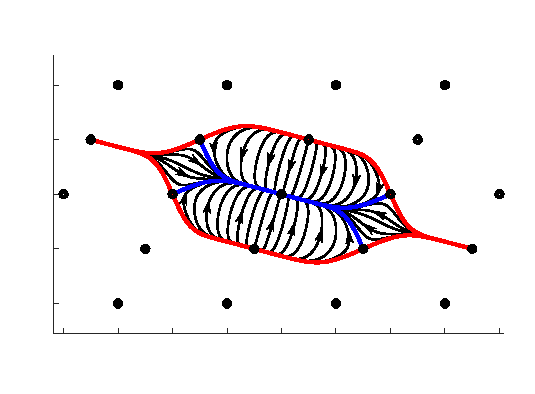
\includegraphics[scale=1.20]{./images/Gradient5.pdf}
\caption{xticks: \; $\displaystyle{-\frac{3\pi}{4}, \; -\frac{\pi}{2},\;  
-\frac{\pi}{4}, \; 0, \; \frac{\pi}{4}, \; \frac{\pi}{2}, \; \frac{3\pi}{4}, \; 
\pi, \; \frac{5}{4} \pi}$ \qquad
yticks: \; $\displaystyle{-\frac{\pi}{2}, \; -\frac{\pi}{4}, \; 0, \; 
\frac{\pi}{4}, \; \frac{\pi}{2}}$}
\end{figure}

\bigskip

\noindent
{\bf Exercise}: Confirm this equation and show that these are critical points 
of $V$.

\bigskip

   We can see from the right hand side of this equation that the set of 
critical points for $V$ forms a lattice in plane.  All of the integer multiples 
of the periods of $V$ (all of the integer multiples of $(\pi,0)^T$ and $(\pi/4, 
\pi/2)^T$) generates a sublattice.

   Within each unit cell of the sublattice there is one minimum for $V$, one 
maximum for $V$ and two saddle points for $V$.

\begin{figure}[ht]
\centering
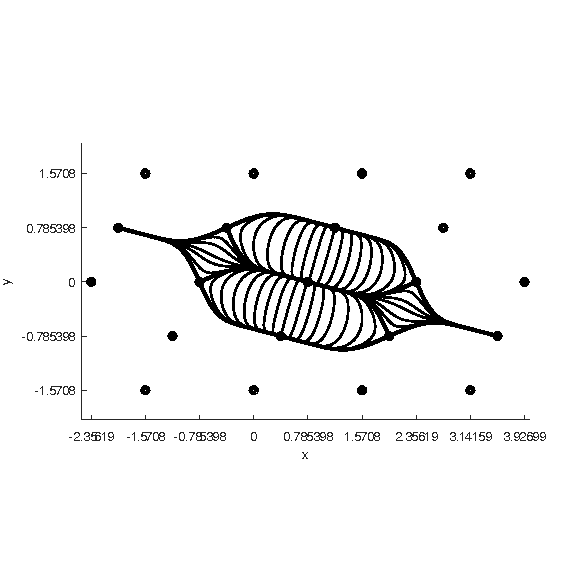
\includegraphics[scale=1.50]{./images/Gradient6.pdf}
\caption{Caption}
\end{figure}

\begin{figure}[ht]
\centering
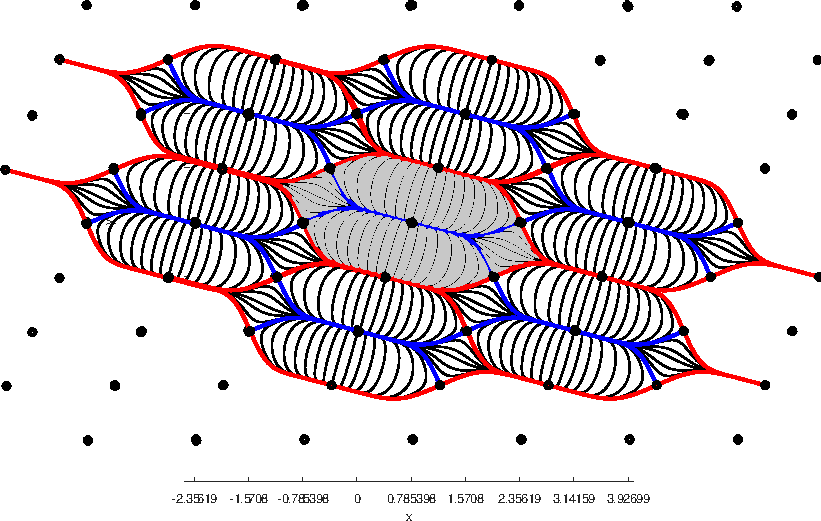
\includegraphics[scale=1.00]{./images/Gradient7.pdf}
\caption{Caption}
\end{figure}

\subsection{Hopfield network with two graded neurons}

   [Used different letters for pedagogy].  We denote the ``input'' of neuron 
$n$ by $x_n$ and the ``output'' by $y_n$.  The ``input-output relation'' (like 
an activation function) is:
\begin{equation*}
   y_n = g(x_n) = \frac{2}{\pi} 
                        \arctan\left( \frac{\pi}{2} \lambda x_n \right)
\end{equation*}
[This function is slightly different from how Hopfield did it in 1984 but it is 
how we did it our papers.]  Its inverse is:
\begin{equation*}
   x_n = g^{-1} (y_n) = \frac{2}{\pi\lambda} 
                        \tan\left( \frac{\pi}{2} y_n \right)
\end{equation*}

   Each stable fixed point will lie in a neighborhood of a vertex of an 
$N$-dimensional hypercube.  The hypercube will be the Cartesian product of the
closed interval $[-1,1] \subset \bf{R}$, \ie $[-1,1]^N$.  Its set of vertices
is $\{-1,1\}^N$.  The number of objects that a Hopfield can detect depends on
the number of neurons in the network.  The more objects we want the network to 
detect the more neurons we need to put in the network.  Experiments indicate
that the number of objects that can be reliably detected by a Hopfield network 
is about $15\%$ of the number of neurons.

   Our example will be a Hopfield network that can distinguish between two 
objects.  We let the vertices be opposite corners of the square
$\{-1,1\}^2$:
\begin{equation*}
\xi_1 = 
\begin{pmatrix}
\xi_{11} \\ \xi_{12}
\end{pmatrix}
=
\begin{pmatrix}
1 \\ -1
\end{pmatrix}
\qquad \mathrm{and} \qquad
\xi_2 = 
\begin{pmatrix}
\xi_{21} \\ \xi_{22}
\end{pmatrix}
=
\begin{pmatrix}
-1 \\ 1
\end{pmatrix}
\end{equation*}
From this we get the weights:
\begin{eqnarray*}
      w_{12} &=& \frac{1}{2} \; \xi_1 \bullet \xi_2
              =  \frac{1}{2} (1 \cdot (-1) + (-1) \cdot 1) = -1 \\
      w_{21} &=& \frac{1}{2} \; \xi_2 \bullet \xi_1
              =  \frac{1}{2} ((-1) \cdot 1 + 1 \cdot (-1)) = -1
\end{eqnarray*}
[I think there is a minor typo in the IJBC paper.  In the cogsci paper we 
referred to the IJBC paper on this.]  The self-weights are both $0$.

  Hopfield's potential function is 
\begin{eqnarray*}
V(x_1, x_2) = &-\,\displaystyle{\frac{1}{2}}& \left(
  \begin{matrix}\begin{pmatrix}y_1 & y_2\end{pmatrix}\\\mbox{}\end{matrix}
  \begin{pmatrix} w_{11} & w_{12} \\ w_{21} & w_{22} \end{pmatrix} 
  \begin{pmatrix} y_1 \\ y_2 \end{pmatrix} \right) \\
%% w_{11} y_1 y_1 + w_{12} y_1 y_2 + w_{21} y_2 y_1 + w_{22} y_2 y_2 \right) \\
&+& \left(\int_0^{y_1} g^{-1}(\chi) \, d\chi 
       + \int_0^{y_2} g^{-1}(\chi) \, d\chi\right) \\
&+& \left(I_1 y_1 + I_2 y_2 \right) \\
V(x_1, x_2) = &-\,\displaystyle{\frac{1}{2}}& \left(
 \begin{matrix}\begin{pmatrix}g(x_1) & g(x_2)\end{pmatrix}\\\mbox{}\end{matrix}
 \begin{pmatrix} 0 & -1 \\ -1 & 0 \end{pmatrix} 
 \begin{pmatrix} g(x_1) \\ g(x_2) \end{pmatrix} \right) \\
&+& \left(\int_0^{g(x_1)} g^{-1}(\chi) \, d\chi 
       + \int_0^{g(x_2)} g^{-1}(\chi) \, d\chi\right) \\
&+& \left(I_1 \, g(x_1) + I_2 \, g(x_2) \right) 
\end{eqnarray*}

\begin{eqnarray*}
V(x_1, x_2) = g(x_1) g(x_2) + \int_0^{g(x_1)} g^{-1}(\chi) \, d\chi 
                            + \int_0^{g(x_2)} g^{-1}(\chi) \, d\chi
             + I_1 \, g(x_1) + I_2 \, g(x_2) 
\end{eqnarray*}
To compute the integrals we compute the indefinite integral:
\begin{eqnarray*}
\int g^{-1}(\chi) \, d\chi  &=& \frac{2}{\pi\lambda} 
                        \int \tan\left( \frac{\pi}{2} \chi \right) \, d\chi \\
~ &=& \frac{2}{\pi\lambda} 
\left( -\frac{2}{\pi} \log\left( \left|\cos\left(\frac{\pi}{2}\chi \right)\right|\right)\right)
= -\frac{4}{\pi^2\lambda} 
\log\left( \left|\cos\left(\frac{\pi}{2}\chi \right)\right|\right)
\end{eqnarray*}
Therefore:
\begin{eqnarray*}
\int_0^{g(x_n)} g^{-1}(\chi) \, d\chi  &=& 
 -\frac{4}{\pi^2\lambda} \left.  \log\left( \left|\cos\left(\frac{\pi}{2}\chi 
\right)\right|\right)\right|_0^{g(x_n)} \\
~ &=& 
 -\frac{4}{\pi^2\lambda}  \log\left( \left|\cos\left(\frac{\pi}{2} g(x_n)
\right)\right|\right)
 +\frac{4}{\pi^2\lambda}  \log\left( \left|\cos(0) \right|\right) \\
~ &=& 
 -\frac{4}{\pi^2\lambda}  \log\left( \left|\cos\left(\arctan\left(
                        \left( \frac{\pi}{2} \lambda x_n \right)\right)\right)\right|\right) + 0
\end{eqnarray*}
We use trig identity for the composition of $\cos$ with $\arctan$.
Since the value of the composition of $\cos$ with $\arctan$ is positive 
everywhere we can drop the absolute signs.
\begin{eqnarray*}
\int_0^{g(x_n)} g^{-1}(\chi) \, d\chi  &=& -\frac{4}{\pi^2\lambda}  \log\left( 
\frac{1}{\sqrt{1 
+ \left(\displaystyle{\frac{\pi}{2}}\lambda x_n\right)^2}} \right) \\
~ &=& -\frac{4}{\pi^2\lambda}  \log\left( \left(1 
+ \left(\displaystyle{\frac{\pi}{2}}\lambda x_n\right)^2\right)^{-\displaystyle{\frac{1}{2}}} \right) \\
~ &=& \frac{2}{\pi^2\lambda}  \log\left( 1 
+ \left(\displaystyle{\frac{\pi}{2}}\lambda x_n\right)^2 \right)
\end{eqnarray*}
The potential function becomes:
\begin{eqnarray*}
V(x_1, x_2) = g(x_1) g(x_2) + 
\frac{2}{\pi^2\lambda} \left(
  \log\left( 1 + \left(\displaystyle{\frac{\pi}{2}}\lambda x_1\right)^2 \right)
+ \log\left( 1 + \left(\displaystyle{\frac{\pi}{2}}\lambda x_2\right)^2 \right)
\right) + I_1 \, g(x_1) + I_2 \, g(x_2) 
\end{eqnarray*}
Note that:
\begin{equation*}
g'(x_n) = \frac{2}{\pi} \dfrac{d}{d x_n} 
                        \arctan\left( \frac{\pi}{2} \lambda x_n \right)
= \frac{2}{\pi} \cdot
\frac{1}{1+ \left(\displaystyle{\frac{\pi}{2}}\lambda x_1\right)^2 }
\cdot \frac{\pi}{2} \lambda
= \frac{\lambda}{1+ \left(\displaystyle{\frac{\pi}{2}}\lambda x_1\right)^2 } 
\end{equation*}
So that
\begin{equation*}
1+ \left(\displaystyle{\frac{\pi}{2}}\lambda x_1\right)^2 = 
\frac{\lambda}{g'(x_n)}
\end{equation*}
The potential function becomes:
\begin{eqnarray*}
V(x_1, x_2) &=& g(x_1) g(x_2) + 
\frac{2}{\pi^2\lambda} \left(
\log\left( \frac{\lambda}{g'(x_1)} \right)
+
\log\left( \frac{\lambda}{g'(x_2)} \right) \right)
+ I_1 \, g(x_1) + I_2 \, g(x_2)  \\
~  &=& g(x_1) g(x_2) + 
\frac{2}{\pi^2\lambda} 
\log\left( \frac{\lambda^2}{g'(x_1) g'(x_2)} \right)
+ I_1 \, g(x_1) + I_2 \, g(x_2)  
\end{eqnarray*}

  To get the negative gradient of the potential we begin with the partial 
derivative with respect to $x_1$: gradient:
\begin{eqnarray*}
\dfrac{dV}{d x_1}(x_1, x_2) &=& g'(x_1) g(x_2) - \frac{2}{\pi^2 \lambda}
\cdot \frac{g''(x_1)}{g'(x_1)}
+ I_1 \, g'(x_1) 
\end{eqnarray*}
Note that:
\begin{eqnarray*}
g''(x_1) &=& \dfrac{d}{d x_1} g'(x_1) = \dfrac{d}{d x_1} 
\frac{\lambda}{1+ \left(\displaystyle{\frac{\pi}{2}}\lambda x_1\right)^2 } \\
~ &=& - \frac{\lambda}{\left(1+ 
\left(\displaystyle{\frac{\pi}{2}}\lambda x_1\right)^2 \right)^2} \cdot 
\left(\frac{\pi \lambda}{2}\right)^2 x_1 \\
 ~ &=& -\frac{\pi^2 \lambda}{4} \, x_1 \left( 
\frac{\lambda}{1+ \left(\displaystyle{\frac{\pi}{2}}\lambda x_1\right)^2 } 
\right)^2 = -\frac{\pi^2 \lambda}{4} \, x_1 g'(x_1)^2
\end{eqnarray*}
Substituting into $dV/dx_1$ gives:
\begin{eqnarray*}
\dfrac{dV}{d x_1}(x_1, x_2) &=& g'(x_1) g(x_2) - \frac{2}{\pi^2 \lambda}
\cdot \left(-\frac{\pi^2 \lambda}{4} \, x_1 \cdot \frac{g'(x_1)^2}{g'(x_1)} \right)
+ I_1 \, g'(x_1) \\
~ &=& g'(x_1) g(x_2) + \frac{1}{2} x_1 g'(x_1) + I_1 \, g'(x_1) \\
~ &=& g'(x_1) \left(\frac{1}{2} x_1  + g(x_2) + I_1\right) 
\end{eqnarray*}
We get $dV/dx_2$ by reversing the subscripts $1$ and $2$.  The ODE for 
gradient descent becomes:
\begin{eqnarray*}
\begin{pmatrix}
\dot{x}_1 \\ \dot{x}_2 
\end{pmatrix}
=
\begin{pmatrix}
g'(x_1) \cdot \left( (1/2) \, x_1  + g(x_2) + I_1\right)  \\[2mm]
g'(x_2) \cdot \left( (1/2) \,  x_2  + g(x_1) + I_2\right) 
\end{pmatrix}
\end{eqnarray*}
If we drop the factors $g'(x_1)$ and $g'(x_2)$ we get the Hopfield's ODE:
\begin{eqnarray*}
\begin{pmatrix}
\dot{x}_1 \\ \dot{x}_2 
\end{pmatrix}
=
\begin{pmatrix}
 (1/2) \, x_1  + g(x_2) + I_1  \\[2mm]
 (1/2) \,  x_2  + g(x_1) + I_2 
\end{pmatrix}
\end{eqnarray*}
Except for the factor $1/2$ which is probably comes from a typo in typesetting.
